\documentclass[paper=a4, fontsize=11pt]{scrartcl} % A4 paper and 11pt font size

\usepackage[T1]{fontenc} % Use 8-bit encoding that has 256 glyphs
\usepackage{fourier} % Use the Adobe Utopia font for the document - comment this line to return to the LaTeX default
\usepackage[english]{babel} % English language/hyphenation
\usepackage{amsmath,amsfonts,amsthm} % Math packages
\usepackage{graphicx}

\usepackage{sectsty} % Allows customizing section commands
\allsectionsfont{\centering \normalfont\scshape} % Make all sections centered, the default font and small caps

\usepackage{fancyhdr} % Custom headers and footers
\pagestyle{fancyplain} % Makes all pages in the document conform to the custom headers and footers
\fancyhead{} % No page header - if you want one, create it in the same way as the footers below
\fancyfoot[L]{} % Empty left footer
\fancyfoot[C]{} % Empty center footer
\fancyfoot[R]{\thepage} % Page numbering for right footer
\renewcommand{\headrulewidth}{0pt} % Remove header underlines
\renewcommand{\footrulewidth}{0pt} % Remove footer underlines
\setlength{\headheight}{13.6pt} % Customize the height of the header

\numberwithin{equation}{section} % Number equations within sections (i.e. 1.1, 1.2, 2.1, 2.2 instead of 1, 2, 3, 4)
\numberwithin{figure}{section} % Number figures within sections (i.e. 1.1, 1.2, 2.1, 2.2 instead of 1, 2, 3, 4)
\numberwithin{table}{section} % Number tables within sections (i.e. 1.1, 1.2, 2.1, 2.2 instead of 1, 2, 3, 4)

\setlength\parindent{0pt} % Removes all indentation from paragraphs - comment this line for an assignment with lots of text

%----------------------------------------------------------------------------------------
%	TITLE SECTION
%----------------------------------------------------------------------------------------

\newcommand{\horrule}[1]{\rule{\linewidth}{#1}} % Create horizontal rule command with 1 argument of height

\title{	
\normalfont \normalsize 
\textsc{University of Copenhagen} \\ [25pt] % Your university, school and/or department name(s)
\horrule{0.5pt} \\[0.4cm] % Thin top horizontal rule
\huge Security Analysis \\ % The assignment title
\horrule{2pt} \\[0.5cm] % Thick bottom horizontal rule
}

\author{Nicolai Willems} % Your name

\date{\normalsize\today} % Today's date or a custom date

\begin{document}

\maketitle % Print the title

\section{Security analysis}
In this assignment, I will examine the security of toll collection point, 
commonly referred to as toll booths. 

\begin{figure}[h]
\centering
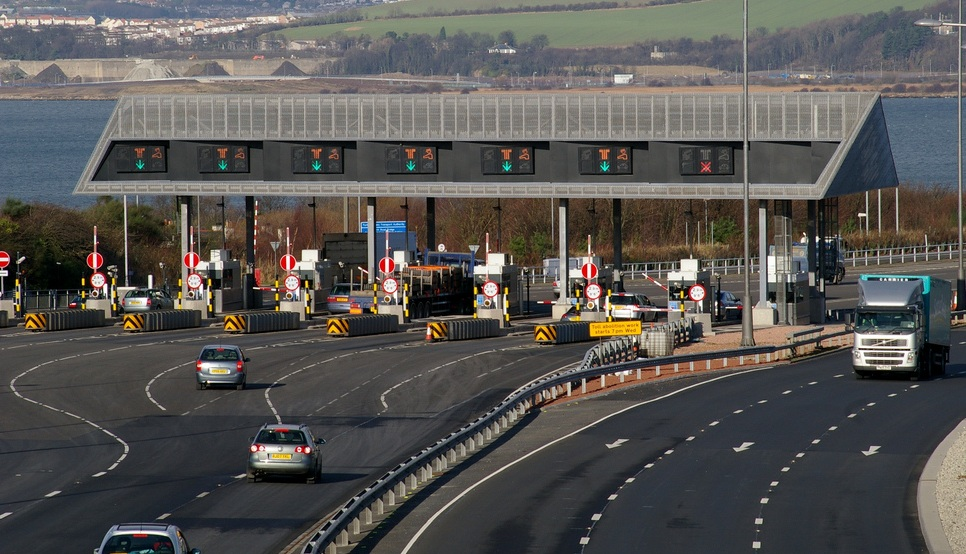
\includegraphics[scale=0.2]{toll_booth}
\caption{A toll booth}
\label{fig:booth}
\end{figure}

Toll booths are usually in place to secure either access to a given road, or
ensure that travellers travelling along the given road pays for distance
travelled. They are also in place between country borders, to keep out unwanted
foreigners.

Historically they have been used by kings and lords, to control roads, either
by sea or by foot, usually in the form of castles at strategic places(ex.
Kronborg).

\subsection{Assets and Security goals}
The main asset in this context is the road or the lands beyond the booth, it 
can be controlled for different reasons, that being security for the traveller,
maintenance of the road or simply limiting access.

Another asset is the actual stand, this is the main enforcing mechanism of the 
system, and is therefore ciritical to its function.

In short the assets are:
\begin{itemize}
\item road/land
\item booth/stand
\end{itemize}

\paragraph{The goal} of the system is to secure that no unwanted traffic is
going through.

\subsection{Adversaries and threats}

\subsection{Weaknesses and defences}

\subsection{Risk analysis}

\subsection{Conclusion}


\end{document}
